
\documentclass[a4paper,UKenglish,cleveref, autoref, thm-restate]{lipics-v2021}

\usepackage{amsmath,amssymb,amsthm}
\usepackage{stmaryrd}
\usepackage{proof}
\usepackage{tikz}
	\usetikzlibrary{calc}

\usepackage{FMC}

\newcommand{\commentout}[1]{}


\bibliographystyle{plainurl}


% - - - - - - - - - - - - - - -


%\newcommand\looppicx[1]{
%\begin{tikzpicture}[thick,x=12pt,y=12pt,outer sep=0pt,inner sep=2pt]
%	\coordinate (m) at (0,0);
%	
%	\begin{scope}[->,>=stealth,anchor=north]
%		\ifx#11
%		\draw (m)--node[pos=0.6,anchor=east]{$\termcolor\scriptstyle{i\vphantom j\,}$} (-1,-2) node {$\vphantom:\typecolor\scriptstyle{p}$};
%		\draw (m)--node[pos=0.6,anchor=west]{\,$\termcolor\scriptstyle{j}$}            ( 1,-2) node {$\vphantom:\typecolor\scriptstyle{q}$};
%		\else
%		\draw (m)--node[pos=0.6,anchor=east]{$\termcolor\scriptstyle{i\vphantom j\,}$} (-1,-2) node {$\vphantom:\typecolor\scriptstyle{\frac p{1-q}}$};
%		\fi
%	\end{scope}
%	
%	\node (x) at (0,-3) {};
%	
%	\coordinate (a) at ( .85,-1.7);% \node[gray,circle,draw,inner sep=0pt,minimum size=2pt] at (a) {};
%	\coordinate (b) at (1.25,-1.6);% \node[gray,circle,draw,inner sep=0pt,minimum size=2pt] at (b) {};
%	
%    	\ifx#10
%		%\draw (m) [rounded corners=20pt] -- (1.25,-2.5) [rounded corners=5pt] -- (1.25,1.5) -- (0,1.5) -- (0,1);
%		\draw[rounded corners=5pt] (m) -- (.5,-1) .. controls (a) and (b) .. (1.25,-.75) -- (1.25,1.5) -- (0,1.5) -- (0,1);
%    	\fi	
%	
%	\node[draw=red,fill=red!10,rounded corners,minimum size=16pt] (M) at (m) {$\term M$};
%	\draw[->,>=stealth] (0,2)--(M);	
%\end{tikzpicture}
%}

\newcommand\looppic[1]{
\vcenter{\hbox{%
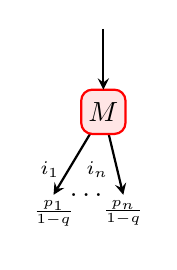
\begin{tikzpicture}[thick,x=18pt,y=15pt,outer sep=0pt,inner sep=2pt]
	\coordinate (m) at (0,0);
	
	\node at (-0.3,-2) {$\dots$};
	
	\begin{scope}[->,>=stealth,anchor=north]
		\draw (m)--node[pos=0.7,anchor=east]{$\termcolor\scriptstyle{i_1\,}$} (-1,-2) node {$\vphantom:\typecolor\scriptstyle{\ifx#11p_1\else\frac{p_1}{1-q}\fi}$};
		\draw (m)--node[pos=0.7,anchor=east]{$\termcolor\scriptstyle{i_n\,}$} (.4,-2) node {$\vphantom:\typecolor\scriptstyle{\ifx#11p_n\else\frac{p_n}{1-q}\fi}$};
	\ifx#11
		\draw (m)--node[pos=0.7,anchor=west]{\,$\termcolor\scriptstyle{j}$}   ( 1,-2) node {$\vphantom:\typecolor\scriptstyle{q}$};
	\fi
	\end{scope}
	
	\node (x) at (0,-3) {};
	
	\coordinate (a) at ( .85,-1.7);% \node[gray,circle,draw,inner sep=0pt,minimum size=2pt] at (a) {};
	\coordinate (b) at (1.25,-1.6);% \node[gray,circle,draw,inner sep=0pt,minimum size=2pt] at (b) {};
	
    	\ifx#10
		%\draw (m) [rounded corners=20pt] -- (1.25,-2.5) [rounded corners=5pt] -- (1.25,1.5) -- (0,1.5) -- (0,1);
		\draw[rounded corners=5pt] (m) -- (.5,-1) .. controls (a) and (b) .. (1.25,-.75) -- (1.25,1.5) -- (0,1.5) -- (0,1);
    	\fi	
	
	\node[draw=red,fill=red!10,rounded corners,minimum size=16pt] (M) at (m) {$\term M$};
	\draw[->,>=stealth] (0,2)--(M);	
\end{tikzpicture}}}
}

\newcommand\markov[1]{\llparenthesis\kern1pt\term{#1}\kern1pt\rrparenthesis}



%==================================================================================================== FRONTMATTER

\title{Types for Almost-Sure Termination in the Functional Machine Calculus}

\author{Ugo {Dal Lago}}{University of Bologna, Italy \and INRIA Sophia Antipolis, France}{ugo.dallago@unibo.it}{https://orcid.org/0000-0001-9200-070X}{}

\author{Willem Heijltjes}{University of Bath, United Kingdom \and \url{http://willem.heijltj.es}}{w.b.heijltjes@bath.ac.uk}{https://orcid.org/0009-0001-8941-1150}{}

\authorrunning{U. Dal Lago and W. Heijltjes}

\Copyright{Ugo Dal Lago and Willem Heijltjes}

\ccsdesc[500]{Theory of computation~Lambda calculus}
\ccsdesc[300]{Theory of computation~Probabilistic computation}

\keywords{probabilistic lambda-calculus, type systems, almost-sure termination}

%\relatedversion{}

%\acknowledgements{Georgina Majury?}

%\nolinenumbers

\hideLIPIcs

\EventEditors{}
\EventNoEds{0}
\EventLongTitle{}
\EventShortTitle{}
\EventAcronym{}
\EventYear{}
\EventDate{}
\EventLocation{}
\EventLogo{}
\SeriesVolume{}
\ArticleNo{}

\newcommand{\UDL}[1]{\textcolor{brown}{Ugo: #1}}

%==================================================================================================== DOCUMENT
\begin{document}

\maketitle

\begin{abstract}
We investigate almost-sure termination in higher-order probabilistic computation through the lens of the functional machine calculus. Our key observation is that iteration  can easily be equipped with a non-zero chance of exiting, thus guaranteeing almost-surely terminating in a simple way. We exploit this insight by shifting attention from recursion to typed iteration, allowing probabilistic behavior to be tracked compositionally at the type level. For the purpose, we introduce a novel probabilistic type system that assigns explicit probability distributions to termination outcomes, and we show that these types soundly guarantee almost-sure termination, even in the presence of higher-order functions. We study the expressive power of the introduced system through an embedding of Markov chains, and prove that \emph{positive} almost-sure termination, while guaranteed at first-order, does not hold at higher-order, in general.
\end{abstract}




%---------------------------------------------------------------------------------------------------- INTRODUCTION

\section{Introduction}

We are interested in applying the tools of the $\lambda$-calculus, in particular confluent reduction and type systems, to probabilistic computation. In~\cite{DalLago-Guerrieri-Heijltjes-2020} we restored confluence to a probabilistic $\lambda$-calculus, the probabilistic event $\lambda$-calculus (PEL), by decomposing probabilistic choice into a \emph{sampling} construct and a \emph{conditional}. Independently in~\cite{Antonelli-DalLago-Pistone-2022} and~\cite{Heijltjes-Majury-2025}, from different inspirations we converged on essentially the same probabilistic type system for the PEL to give lower bounds on the probability of termination. In this paper we further extend the calculus, and develop a type system for \emph{almost-sure termination} (AST): termination with probability one. In doing so, our objective differs from that of many existing works in this area, which aim to capture as many AST programs as possible~\cite{DalLago-Grellois-2019,DalLago-Faggian-Ronchi-2021}, or even to study the feasibility of capturing all such programs~\cite{Kobayashi-DalLago-Grellois-2020}. Instead, we seek to understand the extent to which almost-sure termination can be obtained and explained in a natural manner, possibly using well-established methods, and guaranteed by a minimal extension to simple types. More powerful methods such as dependent types and intersection types may later be used to build on this along standard lines.

We start from the following observation. \emph{Iteration}, generally represented by while-loops, repeats a given function $f$ until a condition is fulfilled. In the typed case, illustrated  below, the function $f$ is required to return a sum $B+A$ where the choice between returning a value $A$ or $B$ represents the condition. Then $\mathsf{iter}\,f$ evaluates $f$, exits on $B$, and repeats on $A$.
\[
\begin{array}{@{}r@{}l@{}}
	f &{}: A \to B+A
\\ \hline
	\mathsf{iter}\,f &{}: A\to B
\end{array}
\]
With the above rule, as with typed fixed-point combinators, typing no longer guarantees termination. However, we observe that if we replace $B+A$ by a probabilistic sum $B \oplus_p A$ with a fixed probability $p\in (0,1]$, i.e.\ the probability of choosing $B$ is non-zero and does not depend on the input, then $\mathsf{iter}\,f$ is \emph{almost-surely terminating} (provided of course that $f$ is itself terminating). This opens a way to approach almost-sure termination via type systems. A crucial question arises: how can we handle a type constructor such as $B\oplus_p A$ within a $\lambda$-calculus with probabilistic choice in a compositional and elegant manner?

These considerations illustrate how probabilistic choice is connected to other imperative features such as sequentiality and iteration. Derived from the PEL, the second author has developed new approach to unifying the $\lambda$-calculus with imperative computation and effects, the \emph{Functional Machine Calculus} (FMC)~\cite{Heijltjes-2023}. Its most recent instance~\cite{Heijltjes-2025-MFPS} features branching sequential computation and iteration, providing an ideal vehicle for our present study. In the FMC each branch of the computation is labelled with a \emph{choice} label $i,j,k,\dots$, which takes the r\^ole of a constant, an exception, a case label, or an exit status. For example, the boolean constants $\bot$ and $\top$ are choice labels. Iteration of a term $\term M$ is written $\term{M^i}$, which evaluates $\term M$ and repeats if $\term M$ chooses $i$, and terminates for any other choice. The calculus encodes a fair probabilistic choice, which we write as $\term{M+N}$.

\begin{example}
The term $\term{(\heads + (\tails + \,i))^i}$ chooses \emph{heads}, the choice label $\heads$, with probability $\frac12$, \emph{tails} $\tails$ with probability $\frac14$, and iterates with probability $\frac14$, to give an overall probability of $\frac 23$ for $\heads$ and $\frac 13$ for $\tails$. We illustrate it pictorially as follows.
\[
	\term{(\heads + (\tails + \,i))^i}
\quad=\quad
\vc{%
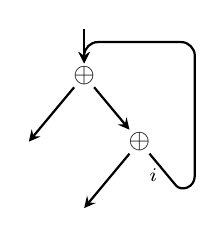
\begin{tikzpicture}[thick,x=20pt,y=24pt,outer sep=0pt,inner sep=1pt]
	\node (x) at (1,2) {$\termcolor\oplus$};
	\node (y) at (2,1) {$\termcolor\oplus$};

	\coordinate (a) at (2.75,0.25); %\node[gray,circle,draw,inner sep=0pt,minimum size=2pt] at (a) {};
	\coordinate (b) at (3   ,0.3);  %\node[gray,circle,draw,inner sep=0pt,minimum size=2pt] at (b) {};
	
	\begin{scope}[->,>=stealth,anchor=north]
	
	\draw (1,2.7)--(x);
	\draw (x)--(y);
	\draw (x) --node[pos=0.6,anchor=south east]{$\termcolor\scriptstyle{\heads}$} (0,1);
	\draw (y) --node[pos=0.6,anchor=south east]{$\termcolor\scriptstyle{\tails}$} (1,0);
	
	\draw[rounded corners=5pt] (y) -- node[pos=0.6,anchor=north east]{$\,\termcolor\scriptstyle{i}$}  
	  (2.5,0.5) .. controls (a) and (b) .. (3,0.7) -- (3,2.5) -- (1,2.5) -- (x);
	\end{scope}
\end{tikzpicture}}
\]
\end{example}

The type system we introduce in this paper, simplified for this introduction to omit inputs and return values, records the probability of terminating with each given choice. A term $\term M$ is typed as follows, indicating that it may choose $i_k$ with probability $p_k$ from choices $i_1$ through $i_n$.
\[
	\term{M : p_1 i_1 * \cdots * p_n i_n }
\]
The type is a probability (sub-)distribution over the choices $\{i_1,\dots,i_n\}$, written as a formal sum. For greater generality, and since our formalism readily incorporates it, we allow the probabilities $p_1$ through $p_n$ to sum to less than one, with the remainder representing a probability of divergence. Terms are almost-surely terminating if the probabilities of their type sum to exactly one.

\begin{example}
The body of our example term, without the loop, has the following type.
\[
	\term{\heads + (\tails + \,i) : \e ~=>~ /12\heads * /14\tails * /14i}
\]
\end{example}

Iteration $\term{M^i}$ removes the choice $i$ from the possible return choices. In the probabilistic setting, the remaining probabilities must then be renormalized to form a distribution. That is, if $i$ has probability $q$, the remaining choices (including divergence) have a total probability of $1-q$, and must be multiplied by $\frac1{1-q}$ to return the total to one. Typing for iteration is then as follows.
\[
\begin{array}{@{}r@{}l@{}}
	\term{M}   &{}: \type{p_1i_1 * \dots * p_ni_n + qj}
\\ \hline \\[-10pt]
	\term{M^j} &{}: \type{/{p_1}{1-q}i_1 * \dots * /{p_n}{1-q}i_n}
\end{array}	
\qquad
\term{M}=\looppic1 \qquad \term{M^j}=\looppic0
\]

\begin{example}
The return type for our example term is given by renormalizing the sub-distribution $\type{/12\heads * /14\tails}$, remaining after removing the element $\type{/14i}$, by multiplying by $\frac 43$, giving the following.
\[
	\term{(\heads + (\tails + \,i))^i : /23\heads * /13\tails}
\]
\end{example}

Types for iteration then correctly give the probabilities for each choice. Consider $\term{M^j}$ where $j$ has probability $q$ in $\term M$. For any other choice $i$ with probability $p$ in $\term M$ the chance of $\term{M^j}$ choosing $i$ is given by the following geometric series, generated by choosing $i$ immediately, after one loop, after two loops, and so forth. The limit of this series is the probability given by the type system.
\[
	p + pq + pq^2 + pq^3 + \cdots ~=~ \frac p{1-q}
\]




The typed calculus achieves the following. A term is guaranteed to terminate with the probabilities of its return type, which is almost-sure termination if the sum probability is one, also in the presence of higher-order probabilistic functions. In a first-order setting it guarantees \emph{positive} almost-sure termination (expected evaluation time is finite), where still it may capture all Markov chains and directly compute their expected output. In the higher-order setting, which gives access to Church numerals, there are examples of \emph{non-positive} or \emph{null} AST.

The probabilistic type system is new for the FMC~\cite{Heijltjes-2025-MFPS}, while the underlying calculus remains essentially the same. It is also a conservative extension of the \emph{sequential} probabilistic event $\lambda$-calculus...

{\color{green}
TO DO:
\\~* decomposition of $N\oplus M$ into $\trm{?a.M}$ and $\trm{MaN}$
\\~* discuss full calculus (with stacks)
\\~* argue this is simple types (Remark~\ref{rem:simple types embed})
\\~* conservativity over previous work (Remark~\ref{rem:probabilistic types embed})
}

%\cite{Hurd-2002}

%while (x>0) { x := x-1 [1/2] x := x+1 }

%  -1 (+) +1 : (=> p1.1 + p2.2 + p3.3 + ...) => (1/2 p1).0 + (1/2 p2).1 + (1/2 p1+p3).2 + (1/2 p2+p3).3 + ...


\bigskip

%---------------------------------------------------------------------------------------------------- BACKGROUND

\section{Related Work}

The type system introduced here can be seen as a conservative extension of the simple type systems studied in \cite{Antonelli-DalLago-Pistone-2022} and \cite{Heijltjes-Majury-2025}. While those systems already featured higher-order functions, they did not account for either iteration or recursion. In the present work, we deliberately choose \emph{iteration} rather than \emph{recursion} in order to keep the framework as simple as possible. Indeed, handling probabilistic recursion poses substantial technical challenges, as it typically requires probabilistic function variables at the type level, effectively leading to the use of dependent types.

Several other works \cite{Avanzini-DalLago-Ghyselen-2019,DalLago-Grellois-2019,DalLago-Padovani-2024,Das-Wang-Hoffmann-2023} introduce type systems that guarantee almost-sure termination (AST) or positive almost-sure termination (PAST) for probabilistic $\lambda$-calculi equipped with recursion. However, these approaches generally prioritise expressive power, often at the expense of conceptual and technical simplicity. A notable exception is the work of the first author with Breuvart and Herrou on AST for extensions of G\"odel’s $\mathbb{T}$~\cite{Breuvart-DalLago-Herrou-2021}. In that setting, however, one endows the underlying calculus either with recursion or with sampling from infinite distributions, rather than with iteration. In contrast, iteration is a fundamentally new ingredient of our approach and plays a central role in preserving simplicity while still capturing nontrivial probabilistic behaviour.

Another related line of research concerns the use of intersection types to characterise AST and PAST properties~\cite{DalLago-Faggian-Ronchi-2021}. Although such characterisations are indeed possible, they come at a significant cost: not only is type inference undecidable, but the resulting type structures are also highly complex. Yet another body of work focuses on the underlying verification problem. Unlike the deterministic case, probabilistic termination is undecidable even for higher-order programs operating over finite datatypes~\cite{Kobayashi-DalLago-Grellois-2020}, e.g., in probabilistic variants of the $\lambda Y$-calculus and higher-order recursion schemes. Our emphasis differs from these approaches, as we deliberately trade expressive power for a simpler and more tractable framework.

Finally, we acknowledge that the calculus introduced here currently has limited expressive power for practical algorithm design. This limitation stems both from the restriction to simple types and from the nature of exit probabilities in the iteration typing rule, which are fixed. A natural direction for future work would be a dependently typed generalisation, reminiscent of Hoare logic. Such an extension could facilitate reasoning about probabilistic termination in interactive theorem proving environments. From this perspective, the extensive body of work on sound verification of almost-sure termination in imperative programs~\cite{FerrerFioriti-Hermanns-2015,McIver-Morgan-Kaminski-Katoen-2018} and probabilistic automata~\cite{Etessami-Yannakakis-2009,Esparza-Kucera-Mayr-2004} also deserves mention. Although motivated by expressiveness and thus fundamentally different in spirit from the present work, this line of research offers many valuable ideas that could potentially be incorporated into the introduced framework.

\commentout{\color{green!66!black}

* Conservative extension of [Curry \&\ Howard meet Borel] and [Simple Types for Probabilistic Termination].

* Uses \emph{iteration} rather than \emph{recursion} to obtain probabilistic typeability. Probabilistic recursion is difficult as it requires probabilistic function variables at type level, essentially using dependent types. Example: probabilistic Church numerals and Y-combinator.

* We believe the observation on typed iterators and almost-sure termination is new.

* Much work on probabilistic termination in verification, but not through type systems, which we believe is new.

* Limited expressive power for real algorithms at present, due to types being simple types. But a dependently typed generalisation would be akin to Hoare logic, and might facilitate probabilistic termination in theorem provers and give natural ways to include termination evidence in typed imperative programming languages.

}

%---------------------------------------------------------------------------------------------------- PROBABILISTIC FMC

\section{The Probabilistic FMC}

The Functional Machine Calculus (FMC)~\cite{Heijltjes-2023,Heijltjes-2025-MFPS} combines the $\lambda$-calculus with imperative programming and effects in the following way. Its point of departure is the (simplified) Krivine Abstract Machine~\cite{Krivine-2007}, a call--by--name operational semantics for the $\lambda$-calculus that evaluates terms in the context of an argument stack, where \emph{application} $M\,N$ pushes $N$, and \emph{abstraction} $\lambda x.M$ pops the head of the stack and substitutes it for $x$. The calculus and the machine are then extended as follows.

\begin{description}
	\item[Effects] The machine is generalised from one to multiple argument stacks or streams, which are then used to model effects: higher-order store as stacks of depth one, input/output as pop-only and push-only streams, and probabilistic choice as a pop-only stream of boolean values. The idea of a probabilistic $\lambda$-calculus that pops from a separate input stream derives from the probabilistic event $\lambda$-calculus~\cite{DalLago-Guerrieri-Heijltjes-2020}, the precursor to the FMC.

	\item[Sequencing] The calculus is extended with imperative \emph{skip} and \emph{sequence} $\term{M;N}$, implemented in standard fashion on the machine with a continuation stack where $\term{M;N}$ pushes $N$ and \emph{skip} pops and executes. This further enables the embedding of Plotkin's call--by--value $\lambda$-calculus, the monadic \emph{return} and \emph{let}-binding of Moggi's computational metalanguage~\cite{Moggi-1991}, and Levy's call--by--push--value~\cite{Levy-2003}.
	
	\item[Control] The calculus is generalised from sequential to branching computation by parameterizing \emph{skip} in a set of \emph{choice} labels $i,j,k,\dots$, each indicating a distinct branch of the computation, and \emph{sequence} to be conditional on a choice $\term{M;i->N}$, continuing with $\term N$ only if $\term M$ terminates with the branch $i$. This is used to model control flow constructions: conditionals, constants, case switches, and exception handling. Iteration is introduced by the construct $\term{M^i}$ which evaluates $\term M$ and iterates on the choice $i$, exiting otherwise, with the semantics $\term{M^i}=\term{M;i->M^i}$.
\end{description}

\noindent
In this way the FMC embeds a minimal but complete imperative programming language, and extends to it two primary features of the $\lambda$-calculus: confluent reduction and simple types. In this paper we consider the \emph{probabilistic FMC}, a fragment of the calculus with \emph{control} and two argument stacks, the regular one for the $\lambda$-calculus and a probabilistic input stream. 

\begin{definition}
The \emph{terms} of the probablistic FMC are given by the following grammar.
\[
\term{M,N} ~\coloneqq~ \term{x} ~\mid~ \term{<x>.M} ~\mid~ \term{[N].M} ~\mid~ \term{i} ~\mid~ \term{M;i->N} ~\mid~ \term{M^i} ~\mid~ \term{?a.M}
\]
\end{definition}

The constructs are: a \emph{variable} $\term x$; a \emph{pop} $\term{<x>.M}$ that binds $\term x$ in $\term M$; a \emph{push} $\term{[N].M}$; a \emph{choice} $\term i$; a \emph{case} $\term{M;i->N}$; a \emph{loop} $\term{M^i}$; and a \emph{generator} $\term{?a.M}$ which binds the variable $\term a$ in $\term M$.

The $\lambda$-calculus embeds by letting $\lambda x.M=\term{<x>.M}$ and $M\,N=\term{[N].M}$. The generator $\term{?a.M}$ is rendered as $\term{`{\mathsf{rnd}}<a>.M}$ in other presentations of the FMC, as a parameterised pop construct. Probabilistic choice embeds as follows, where the \emph{case} construct associates left, $\term{M; i->N ; j->P}=\term{(M; i->N) ; j-> P}$.
\[
	\term{M+N} ~=~\term{?a.a ; \top->M ; \bot->N }
\]
In this construction, first $\term{?a}$ pops a boolean value $\term\top$ or $\term\bot$ from a probabilistic stream and substitutes it for $\term a$. The remainder then selects the relevant branch by the semantics of the \emph{case} construct, given by the equations $\term{i;i->M}=\term M$ and $\term{j;i->M}=\term j$ for $i\neq j$. We reserve the choice labels $\top$ and $\bot$ for the purpose of encoding probabilistic choice: here, if $\term M$ were allowed to choose $\term\bot$, that would incorrectly trigger $\term N$ after evaluating $\term M$.

% - - - - - - - - - - - - - - - - - - - - - - - - - - - - - - Abstract machine
\subsection*{The Operational Semantics}

The Probabilistic FMC can be given meaning via an abstract machine whose state consist of the term under evaluation, two stacks (namely, the continuation stack and the evaluation stack) and a trace. The trace records the outcomes of future probabilistic choice instructions, thereby rendering the machine effectively deterministic. More formally, the machine evaluates a term $\term M$ in a state $(t,S,\term M,K)$, in the context of three stacks: 
\begin{itemize}
	\item A \emph{trace} $t$, a stack of boolean values $\top$ and $\bot$, from which $\term{?a.M}$ pops. 
	\item An \emph{argument stack} $S$ of terms, where $\term{[N].M}$ pushes $\term N$, and $\term{<x>.M}$ pops the head $\term N$ and continues as $\term{\{N/x\}M}$, the capture-avoiding substitution of $\term N$ for $\term x$ in $\term M$.
	\item A \emph{continuation stack} $K$, a stack of cases $\term{i->M}$, where $\term{M;i->N}$ pushes $\term{i->N}$ and $\term{M^i}$ pushes $\term{i->M^i}$. A choice $\term j$ pops the head $\term{i->M}$ and continues as $\term M$ if $i=j$, and as $\term j$ otherwise.
\end{itemize}

\begin{definition}
The \emph{functional abstract machine} is given by the following data. \emph{Traces}, \emph{argument stacks}, and \emph{continuation stacks} are as follows.
\[
    r,s,t ~\coloneqq~ \e ~\mid~ \bot\,t ~\mid~ \top\,t   \qquad\quad 
    R,S,T ~\coloneqq~ \e ~\mid~ S\,\term M               \qquad\quad 
    K,L   ~\coloneqq~ \e ~\mid~ (\term{i->M})\,K
\]
The \emph{states} of the machine are four-tuples $(t,S,\term M,K)$. Its \emph{steps} or \emph{transitions} are given in Figure~\ref{fig:machine}. A \emph{run} of the machine is a sequence of steps, written with a double line as below. A \emph{successful} run is one terminating in a \emph{final state} $\state\e Ti\e$ with a choice term $\term i$ and empty trace and continuation stack.
\[ 
	\step= sSMK tTNL
\]
\end{definition}

% - - - - - - - - - - Machine figure
\begin{figure}
\[
\begin{array}{lccr}
	  \mathsf{push}     & \step- t S {[N].M} K             t {S\,\term N} M K
	                    & \step- t S i {(\term{i->M})\,K}  t S M K                    & \mathsf{select}
\\ \\ \mathsf{pop}      & \step- t {S\,\term N} {<x>.M} K  t S {\{N/x\}M} K
	                    & \step- t S i {(\term{j->M})\,K}  t S i K                    & \mathsf{reject}
\\ \\ \mathsf{sequence} & \step- t S {M;i->N} K            t S M {(\term{i->N})\,K}
	                    & \step- t S {M^i} K               t S M {(\term{i->M^i})\,K} & \mathsf{iterate}
\\ \\ \mathsf{sample}   & \step- {\top\,t} S {?a.M} K      t S {\{\top/a\}M} K
                        & \step- {\bot\,t} S {?a.M} K      t S {\{\bot/a\}M} K
\end{array}
\]
\caption{The Abstract Machine}
\label{fig:machine}
\end{figure}
% - - - - - - - - - - 


In addition to the machine we use a big-step operational semantics, in the form of an inductively defined evaluation relation $(\evalarrow)$, which describes the successful runs of the machine directly.

\begin{definition}
The \emph{evaluation} relation has statements $\eval tSM Ti$ and is defined inductively by the following rules.
\[
\begin{array}{ccc}
     \infer[\Rax]  {\eval \e Si Si}{}
   & \infer[\Rsel] {\eval {rs}R{M;i->N} Tj }{\eval rRM Si & \eval sSN Tj}
   & \infer[\Rrej] {\eval rR{M;i->N} Sj }{\eval rRM Sj}
\\\\ \infer[\Rpush]{\eval sS{[N].M} Ti}{\eval s{S\,\term N}M Ti}
   & \infer[\Rloop]{\eval {rs}R{M^i} Tj }{\eval rRM Si & \eval sS{M^i} Tj}
   & \infer[\Rexit]{\eval rR{M^i} Sj }{\eval rRM Sj} 
\\\\ \infer[\Rpop] {\eval t{S\,\term N}{<x>.M} Ti}{\eval tS{\{N/x\}M} Ti}
   & \infer[\Rbot] {\eval {\bot\,t}S{?a.M} Ti}{\eval tS{\{\bot/a\}M} Ti}
   & \infer[\Rtop] {\eval {\top\,t}S{?a.M} Ti}{\eval tS{\{\top/a\}M} Ti}
\end{array}
\]
\end{definition}
The machine and the big-step evaluation relation can be put in correspondence as follows.
\begin{proposition}[{\cite[Proposition 5.4]{Heijltjes-2025-MFPS}}]
Evaluation characterizes successful machine termination:
\[
\eval tSMTi \quad \iff \quad \step= tSM\e \e Ti\e
\]
\end{proposition}


% - - - - - - - - - - - - - - - - - - - - - - - - - - - - - - Probabilistic evaluation

\subsection*{Probabilistic Evaluation}

The FMC as defined above is still deterministic: it externalises the probabilistic component of evaluation to the input trace $t$ and how this is generated. Here, we will define \emph{probabilistic} evaluation by considering distributions of machine runs over distributions of traces $t$. 

A \emph{frontier} $F$ is a (possibly infinite) set of traces such that no element in $F$ is a prefix of another. The \emph{probability} $\pr F$ of a frontier $F$ is the sum probability of its traces.
\[
\begin{array}{l@{}l}
	    \pr t &~=~ (\frac12)^{|t|} \quad\text{where $|t|$ is the length of $t$}
\\[5pt]	\pr F &~=~ \sum_{t\in F}\pr t
\end{array}
\]

\begin{example}
\label{ex:frontier}
The set of traces $\{ (\bot^n)\top\mid n\in \N \} = \{ \top,\bot\top,\bot\bot\top,\dots\}$ is a frontier with probability $1$.
\end{example}


A \emph{return family} $\DS$ gives the result of successfully evaluating a term for every trace in a given frontier $F$, collecting for each $t\in F$ a return stack $S_t$ and choice $i_t$ as the pair $(S_t,i_t)_t$ indexed with $t$. The frontier $F$ over which $\DS$ is defined is written $\floor\DS=F$, and the \emph{probability} of a return family is that of its frontier, $\pr\DS = \pr{\floor\DS}$.
\[
	\DS,\DT~\coloneqq~\{ (S_t,i_t)_t \}_{t\in F}
\]

\begin{definition}
A \emph{probabilistic evaluation} $\Eval SM\DT$ of a term $\term M$ in the context of a stack $S$ to a return family $\DT$ is given by the evaluation of $\term M$ and $\term S$ with each $t\in F$, as follows.
\[
	\Eval SM{\{ (T_t,i_t)_t \}_{t\in F}} \iff \forall t\in F.~(\eval tSM {T_t}{i_t})
\]
\end{definition}

\begin{example}
For the term $\term M=\term{(\heads + (\tails + \,i))^i}$ of the introduction we have $\Eval \e M \DT$ for the following return family $\DT$ over the frontier of Example~\ref{ex:frontier}.
\[
	\DT~=~\{ (\e,\heads)_t \mid t = (\bot^{2n})\top,~n\in\N~\} \cup \{ (\e,\tails)_t \mid t = (\bot^{2n+1})\top,~n\in\N~\}
\] 
\end{example}

Observe that evaluation is closed under inclusion: if $\Eval RM\DT$ and $\DS\subseteq\DT$ then $\Eval RM\DS$. An evaluation $\Eval SM\DT$ gives a lower bound of $\pr{\DT}$ for the probability of termination of a term $\term M$ in the context of a stack $S$.

\begin{definition}
The \emph{probability of termination} of a term $\term M$ in the context of a stack $S$ is the largest probability $\pr{\DT}$ for any $\DT$ such that $\Eval SM\DT$.
\end{definition}

To work with return families we use the following notation. The \emph{sum} of two return families $\DS+\DT$ is defined if they have disjoint frontiers, $\floor\DS\cap\floor\DT=\varnothing$, as the union of their underlying sets $\DS\cup\DT$. Likewise, \emph{inclusion} between families $\DS\subseteq\DT$ is inclusion as sets. We define the following notions below: $s\pfx F$ and $s\pfx\DS$ add $s$ as a prefix to every trace $t$ in $F$, respectively in $\DS$, and $S\,\DT$ prefixes every stack in $\DT$ with $S$; $\DS\only i$ restricts a family to the choice $i$ and $\DS\less i$ excludes the choice $i$; and $\stk\DS$ collects the stacks in $\DS$ as a set. 
\[
\begin{array}{r@{}l@{\qquad\qquad}r@{}l}
		s\pfx F    &{}~=~\{ \, st \mid t\in F \,\}                & \DS\only i &{}~=~\{ \,(S,j)_t \in \DS \mid j=i \,\} 
\\[5pt] s\pfx\DS   &{}~=~\{ \,(S,i)_{st} \mid (S,i)_t \in \DS\,\} & \DS\less i &{}~=~\{ \,(S,j)_t \in \DS \mid j\neq i \,\}
\\[5pt] S\,\DT     &{}~=~\{ \,(S\,T,i)_t \mid (T,i)_t \in \DT\,\} & \stk\DS    &{}~=~\{ \,S \mid (S,i)_t \in \DS\,\}
\end{array}
\]
We will freely use the following equations.
\[
	\floor{s\pfx\DS} = s\pfx\floor\DS    \qquad\quad
	\pr{s\pfx\DS}    = \pr s\times\pr\DS \qquad\quad
	\pr{\DS+\DT}     = \pr\DS + \pr\DT
\]


%---------------------------------------------------------------------------------------------------- TYPES

\section{Types}

Types for the FMC describe the input/output behaviour of the machine. In the deterministic case, a type $\type t$ is of the form below left, where the type vector $\type{!s}=\type{s_1 .. s_k}$ types the input stack on the machine, and the type vectors $\type{!t_m}$ type the return stack for each choice $i_m$. The type indicates that given an input stack $S:\type{!s}$ the machine will return some choice $i_m$ and stack $T:\type{!t_m}$. For the probabilistic case we replace the formal sum of the return type with a probability distribution, adding a probability $p_m$ for each summand as below right. For probabilities, we use rationals in $[0,1]$.
\[
	\type{!s ~=>~!t_1.i_1 + .. + !t_n.i_n} \qquad\qquad
	\type{!s ~=>~!t_1.p_1i_1 * .. * !t_n.p_ni_n}
\]
We will formalize the return type as \emph{distribution type}, a family in a finite set $I$ of choice labels, with a type vector $\type{!t_i}$ and a probability $p_i$ for each $i\in I$ such that the sum probability over all $p_i$ is at most one. It is thus a combination of a deterministic sum type, the family of type vectors $\type{!t_i}$, and a probability (sub-)distribution over $I$, the family of probabilities $p_i$.

\begin{definition}
\emph{Types}, \emph{stack types}, and \emph{distribution types} are given as follows.
\[
\begin{array}{l@{\qquad}r@{~\coloneqq~}l}
	\text{types}	            & \type{s,t} & \type{!t => d}
\\	\text{stack types}          & \type{!t}  & \type{t_1..t_n}
\\  \text{distribution types}   & \type{g,d} & \type{\{(!t_i,p_i)_i\}_{i\in I}}\quad\text{where}\quad\sum_{i\in I}p_i\leq 1
\end{array}
\]
\end{definition}

We introduce the following notation to work with distribution types. The \emph{basis} of a distribution type $\type d$, the set of choices $I$ over which it is defined, is $\floor{\type d}=I$. To recover the informal notation at the start of the section, we define the \emph{singleton} distribution type $\type{!t.pi}=\type{\{(!t,p)_i\}}$ and the \emph{sum} $\type{g*d}=\type{g\cup d}$ of distribution types over disjoint bases $\floor{\type g}\cap\floor{\type d}$. The \emph{probability} $\pr{\type d}$ of a distribution type is the sum over its probabilities $p_i$. Below, $\type{!s\,d}$ prefixes the type vector $\type{!s}$ to each $\type{!t}$ in $\type d$, and $\type{q.d}$ multiplies each probability $p_i$ in $\type d$ by the probability $q$. Below right, $\type{d|I}$ restricts $\type d$ to the choices in $I$, and $\type{d-I}$ removes them.
\[
\begin{array}{r@{}l@{\qquad\qquad}r@{}l}
	    \type{q.d}   &{}~=~ \type{\{    (!t,qp)_i \mid (!t,p)_i\in d\, \}}  & \type{d|I} &{}~=~ \type{\{ (!t.p)_i \in d \mid i\in I\,\}}
\\[5pt]	\type{!s\,d} &{}~=~ \type{\{ (!s\,!t,p)_i \mid (!t,p)_i\in d\, \}}  & \type{d-I} &{}~=~ \type{\{ (!t.p)_i \in d \mid i\notin I\,\}}
\end{array}
\]
Finally, the \emph{merger} $\type{g++d}$ of two distribution types is defined if for every $i\in\floor{\type g}\cap\floor{\type d}$ they have the same type vector $\type{!t_i}$, and is as follows.
\[
	\type{g++d} ~=~ \type{ \{ (!t,p+q)_i \mid i\in {\floor\gamma}\cup{\floor\delta}~`,~(!t,p)_i \in g~`,~(!t,q)_i\in d\}~+~g-{\floor\delta}~+~d-{\floor\gamma} }
\]

\begin{definition}
The \emph{typed probabilistic FMC} is given by the typing rules in Figure~\ref{fig:types}, where a context $\term{G}=\term{x_1:t_1,,x_n:t_n}$ is a finite function from variables to types written as a sequence, and typing judgment $\term{G |- M:t}$ assigns a term $\term M$ the type $\type t$ in the context $\term G$.
\end{definition}

% - - - - - - - - - - Types figure
\begin{figure}
\[
\begin{array}{l@{\qquad}c@{\qquad}c@{\qquad}r}
      \mathsf{variable}  & \vc{\infer{\term{G, x:t |- x:t}}{}}
                         & \vc{\infer{\term{G |- M : !s => 0 . d}}{}}                                 & \mathsf{zero}
\\ \\ \mathsf{pop}       & \vc{\infer{\term{G |- <x>.M : r\,!s => d}}{\term{G , x:r |- M: !s => d}}}
                         & \vc{\infer{\term{G |- [N].M : !s => d}}
                                     {\term{G |- N:r} && \term{G |- M : r\,!s => d}}}                 & \mathsf{push}
\\ \\ \mathsf{choice}    & \vc{\infer{\term{G |- i: !s => !s.1i}}{}}
                         & \vc{\infer{\term{G |- M;i->N : !r => g ++ (p . d)}}
                                     {\term{G |- M: !r => g * !s.pi} && 
                                      \term{G |- N: !s => d}}}                                        & \mathsf{sequence}
\\ \\ \mathsf{expand}    & \vc{\infer{\term{G |- M: !s\,!r => !r\,d}}{\term{G |- M: !s => d}}}
                         & \vc{\infer{\term{G |- M^i: !s => /1{1-p} . d}}
                                     {\term{G |- M: !s => d * !s.pi} && (p\neq 1)} }                  & \mathsf{iterate}    
\\ \\ \mathsf{sample}    & \multicolumn{2}{c}{
                           \vc{\infer{\term{G |- ?a.M : !r => (/12 . g) ++ (/12 . d)}}
                                     {\term{G , a: \e => \e.1\top |- M: !r => g} && 
                                      \term{G , a: \e => \e.1\bot |- M: !r => d}}}
                          }
\end{array}
\]
\caption{The typed probabilistic FMC}
\label{fig:types}
\end{figure}
% - - - - - - - - - -

\begin{example}
The probabilistic sum $\term{M+N}=\term{?a.a ; \top->M ; \bot->N }$ is typed as follows.
\[
\infer{ \term{|- ?a.a ; \top -> M ; \bot -> N : !t ~=>~ /12.g ~++~ /12.d} }{
 \infer{ \term{|- ?a.a ; \top -> M : !t ~=>~ !t./12\top ~*~ /12.d } }{
  \infer{ \term{|- ?a.a : !t ~=>~ !t./12\top ~*~ !t./12\bot} }{
   \infer{ \term{|- ?a.a : \e ~=>~ \e./12\top ~*~ \e./12\bot} }{
    \infer{ \term{ a: \e => \e.1\top |- a: \e => \e.1\top} }{}
    &&
    \infer{ \term{ a: \e => \e.1\bot |- a: \e => \e.1\bot} }{}
  }} &
  \term{|- M : !t => g}
 } &
 \term{|- N : !t => d}
}
\]
Using this as an admissible typing rule, our running example is typed as follows.
\[
\infer{ \term{|- (\heads + (\tails + \,i))^i : \e ~=>~ \e./23\heads ~*~ \e./13\tails} }{
 \infer{ \term{|- \heads + (\tails + \,i) : \e ~=>~ \e./12\heads ~*~ \e./14\tails ~*~ \e./14i} }{
  \infer{ \term{|- \heads : \e ~=>~\e.1\heads}}{}
  &&
  \infer{ \term{|- \tails + \,i : \e ~=>~ \e./12\tails ~*~ \e./12i } }{
   \infer{ \term{|- \tails : \e ~=>~\e.1\tails}}{}
   &&
   \infer{ \term{|- i : \e ~=>~\e.1i}}{}
}}}
\]
\end{example}

\begin{remark}
\label{rem:simple types embed}
The type system is a conservative extension of simple types for the $\lambda$-calculus. These embed as follows, using a single default choice $\star$ (see also~\cite{Heijltjes-2023,Heijltjes-Majury-2025,Heijltjes-2025-MFPS}). For these types, the typing rules for $\mathsf{variable}$, $\mathsf{pop}$, and $\mathsf{push}$ are those of the simply typed lambda-calculus.
\[
	\typ{t_1 \to \dots \to t_n \to o} \quad=\quad \type{t_1 \dots t_n => \e.1\star}
\]
\end{remark}

\begin{remark}
\label{rem:probabilistic types embed}
The type system is also a conservative extension of those of our previous work on probabilistic termination~\cite{Antonelli-DalLago-Pistone-2022,Heijltjes-Majury-2025}. Using the notation of~\cite{Heijltjes-Majury-2025}, simple probabilistic types are simple types over the rationals between $0$ and $1$ as the set of base types, and embed as follows, where $p\in\mathbb{Q}\cap[0,1]$ and $\star$ is again the single available choice label.
\[
	\typ{t_1 \to \dots \to t_n \to p} \quad=\quad \type{t_1 \dots t_n => \e.p\star}
\]
\emph{Sequential probabilistic types}~\cite{Heijltjes-Majury-2025} are the restriction of the present system to the choice $\star$.
\[
	\typ{!s} \overset{p}{\Rightarrow} \typ{!t} \quad=\quad \type{!s => !t.p\star}
\]
\end{remark}

% - - - - - - - - - - - - - - - - - - - - - - - - - - - - - - Almost sure termination
\subsection*{Almost-Sure Termination}

The intended meaning of the type system is that if $\term{|- M: \e => d}$ (i.e.\ $\term M$ requires no inputs to run on the machine) then the probability of termination for $\term M$ is at least $\pr{\type d}$. We will establish this using a reducibility argument in the style of Tait~\cite{Tait-1967}, called \emph{runnability} since it uses the machine rather than reduction. 
The runnability predicate directly interprets the meaning of types: a runnable term of type $\term{M:!s => d}$, given a stack $S$ of runnable terms for the types in $\type{!s}$, will probabilistically evaluate to a runnable return family $\DT$ for the type $\type{d}$, with the key property that $\pr{\DT}\geq\pr{\type d}$.

\begin{definition}
The set $\RUN{t}$ of \emph{runnable terms} for a type $\type t$ is defined as the set of closed terms
\[
	\RUN{!s => d} = \{ \term M ~\mid~ \forall S \in\RUN{!s}.~\exists\DT\in\RUN{d}.~\Eval SM\DT~\}
\]
where the runnable sets for stack types $\type{!t}$ and distribution types $\type{d}$ are as follows.
\[
    \RUN{t_1..t_n} = \{ \e\,\term{M_1}\dots \term{M_n} \mid \term{M_i}\in\RUN{t_i} \}
\]
\[
	\RUN{\{(!t_i,p_i)_i\}_{i\in I}} = \{ \DT \mid \forall i\in I.~\stk{\DT\only i}\subseteq\RUN{!t_i}~\wedge~\pr{\DT\only i}\geq p_i~\}
\]
\end{definition}

To work with open terms, a \emph{substitution map} $\mu$ is a finite function from variables to terms, applied to a term as $\term{\mu M}$ which replaces every free variable $x$ in the domain of $\mu$ with the term $\term{\mu(x)}$. for a context $\Gamma=\term{x_1:t_1,..,x_n:t_n}$ the set $\SRUN{G}$ is a set of substitution maps $\mu$ that assigns each $x_i$ a runnable term $\term M\in\RUN{t_i}$, as follows.
\[
	\SRUN{G}~=~\{ \mu \mid \forall\term{x:t}\in\Gamma.~\term{\mu(x)}\in\RUN{t}\}
\]
We are now ready to prove the \emph{runnability lemma}, that typed terms are runnable.

% - - - - - - - - - - - - - - -
\begin{lemma}
\label{lem:run}
If $\term{G |- M:t}$ and $\mu\in\SRUN{G}$ then $\term{\mu M}\in\RUN{t}$.
\end{lemma}

\begin{proof}

By induction on the typing derivation.

\begin{itemize}

	% Variable
	\item \emph{Variable:} 
\[
\infer{\term{G, x:t |- x:t}}{}
\]
By the definition of $\SRUN{G}$ we have $\term{\mu x}\in\RUN t$.

	% Choice
	\item \emph{Choice:}
\[
\infer{\term{G |- i: !s => !s.1i}}{}
\]
Let $S\in\RUN{!s}$ and note that $\term{\mu i}=\term i$ for any $\mu$. We have the evaluation $\eval\e Si Si$ for the empty trace. Then for the frontier $\{\e\}$ we have $\Eval Si{\{(S,i)_\e\}}$, with the singleton return family of $S$ and $i$ for the empty trace. Since $S\in\RUN{!s}$ and $p(\e)=1$ it follows that $\{(S,i)_\e\}\in\RUN{!s.1i}$.

	% Zero
	\item \emph{Zero}
\[
\infer{\term{G |- M : !s => 0 . d}}{}
\]
For any $S$ and $\mu$ we have $\Eval S{\mu M}\varnothing$. Since $\varnothing\subseteq\RUN{!t}$ for any $\type{!t}$ and $\pr{\varnothing\only i}\geq 0$ for any $i$ we have $\varnothing\in\RUN{0.d}$.

	% Expand
	\item \emph{Expand:}
\[
\infer{\term{G |- M: !s\,!r => !r\,d}}{\term{G |- M: !s => d}}
\]
Let $R\in\RUN{!r}$, $S\in\RUN{!s}$, and $\mu\in\SRUN{G}$. The inductive hypothesis gives the evaluation $\Eval SM\DT$. For each $(T,i)_t\in\DT$ we have the evaluation below left. By induction on the evaluation relation $\evalarrow$ we get the evaluation below right.
\[
\eval tS{\mu M}Ti
\qquad\qquad
\eval t{RS}{\mu M}{RT}i
\]
This gives $\Eval{RS}{\mu M}{R\,\DT}$. Since $R\in\RUN{!r}$ and $\stk{\DT\only i}\subseteq\RUN{!t_i}$, where $\type{!t_i}$ is the type for $i$ in $\type d$, we have $\stk{R\,\DT\only i} \subseteq \RUN{!r\,!t_i}$. Since also $\pr{R\,\DT\only i}=\pr{\DT\only i}\geq p_i$ we have $R\,\DT\in\RUN{!r\,d}$. 

	% Push
	\item \emph{Push:} 
\[
\infer{\term{G |- [N].M : !s => d}}{\term{G |- N:r} && \term{G |- M : r\,!s => d}}
\]
Let $S\in\RUN{!s}$ and $\mu\in\SRUN{G}$. By induction we have $\term{\mu N}\in\RUN{r}$ and $\term{\mu M}\in\RUN{r\,!s=>d}$, and for the latter the evaluation $\Eval {S\,\term{\mu N}}{\mu M}\DT$. Then for every $(T,i)_t\in \DT$ we have the evaluation below left, from which we construct the derivation below right.
\[
	\eval t{S\,\term{\mu N}}{\mu M}Ti
\qquad\qquad
	\vc{\infer[\Rpush]{ \eval tS{\mu([N].M)} Ti }{ \eval t{S\,\term{\mu N}}{\mu M} Ti } }
\]
Then $\Eval S{\mu([N].M)}\DT$ and $\term{\mu([N].M)}\in\RUN{!s => d}$.

	% Pop
	\item \emph{Pop:}
\[
\infer{\term{G |- <x>.M : r\,!s => d}}{\term{G , x:r |- M: !s => d}}
\]
Let $S\in\RUN{!s}$, $\term N\in\RUN r$, and $\mu\in\SRUN{G}$. Let $\mu'=\mu\{\term N/x\}$, the substitution map that sends $x$ to $\term N$ and every other variable $y$ to $\mu y$, so that $\mu'\in\SRUN{G,x:r}$. By induction we have $\Eval S{\mu'M}\DT$, given by the evaluation below for every $(T,i)_t\in\DT$, from which we construct the evaluation below right.
\[
	\eval tS{\mu'M} Ti
\qquad\qquad
	\vc{ \infer[\Rpop]{ \eval t{S\,\term{N}}{\mu(<x>.M)}Ti } {\eval tS{\mu'M}Ti} } 
\]
Then $\Eval{S\,\term N}{\mu(<x>.M)}\DT$ and $\term{\mu(<x>.M)}\in\RUN{r\,!s=>d}$.


	% Sample
	\item \emph{Sample:}
\[
\infer{\term{G |- ?a.M : !r => (/12 . g) ++ (/12 . d)}}{\term{G , a: \e => \e.1\top |- M: !r => g} && \term{G , a: \e => \e.1\bot |- M: !r => d}}
\]
Let $R\in\RUN{R}$ and $\mu\in\SRUN{G}$. Define $\mu_\top=\mu\{\term\top/a\}$ and $\mu_\bot=\mu\{\term\bot/a\}$ so that $\mu_\top\in\SRUN{G , a: \e => \e.1\top}$ and $\mu_\bot\in\SRUN{G , a: \e => \e.1\bot}$. By induction we have return families $\DS$ and $\DT$ where $\Eval R{\mu_\top M}\DS$ and $\Eval R{\mu_\bot M}\DT$, given by the following evaluations for every $(S,i)_s\in\DS$ and $(T,j)_t\in\DT$.
\[
\eval sR{\mu_\top M}Si \qquad\qquad  
\eval tR{\mu_\bot M}Tj
\]
For these we have the following derivations.
\[
\infer[\Rtop]{ \eval{\top\,s}R{\mu(?a.M)}Si }{ \eval sR{\mu_\top M}Si } \qquad
\infer[\Rbot]{ \eval{\bot\,t}R{\mu(?a.M)}Tj }{ \eval tR{\mu_\bot M}Tj }
\]
Then for $\DU=(\top\pfx\DS)\cup(\bot\pfx\DT)$ we have $\Eval S{\mu(?a.M)}\DU$. It remains to show that $\DU\in\RUN{/12.g ++ /12.d}$. For any indexed pair in $\type{/12.g ++ /12.d}$, by the definition of $(\type{++})$ we have three cases.
\begin{itemize}
	\item $\type{(!t,/12p+/12q))_i}$ where $i\in\floor{\type g}\cap\floor{\type d}$, $\type{(!t.p)_i}\in\type g$ and $\type{(!t.q)_i}\in\type d$. Then since $\stk{\DS\only i}\subseteq\RUN{!t}$ and $\stk{\DT\only i}\subseteq\RUN{!t}$ we have $\stk{\DU\only i}\subseteq\RUN{!t}$, and since $\pr{\DS\only i}\geq p$ and $\pr{\DT\only i}\geq q$ we have $\pr{\DU\only i}=\pr{\top\pfx\DS\only i}+\pr{\bot\pfx\DT\only i}\geq \frac 12p+\frac 12q$.
	\item $\type{(!t,/12p)_i}$ in $\type{/12.g-{\floor\delta}}$. Since $\stk{\DS\only i}\subseteq\RUN{!t}$ we have $\stk{\DU\only i}\subseteq\RUN{!t}$, and since $\pr{\DS\only i}\geq p$ we have $\pr{\DU\only i}=\pr{\top\pfx\DS\only i}\geq\frac 12p$.
	\item The case for $\type{/12.d-{\floor\gamma}}$ is analogous to the previous.
\end{itemize}

	% Sequence
	\item \emph{Sequence:} 
\[
\infer{\term{G |- M;i->N : !r => g ++ p.d}}
      {\term{G |- M: !r => g * !s.pi} && 
       \term{G |- N: !s => d}}
\]
Let $R\in\RUN{!r}$ and $\mu\in\SRUN{G}$. By induction we have $\term{\mu M}\in\RUN{!r => g * !s.pi}$ and $\Eval R{\mu M}\DS$. Let this be given by an evaluation for each $(S,j)_s\in\DS$ of the form below left. For each $(S,j)_s$ where $j=i$ we have $S\in\RUN{!s}$, and by induction on $\term{N}$ a return family $\DT_s$ such that $\Eval S{\mu N}{\DT_s}$. Let this be given by the evaluation below right for each $(T,k)_t\in\DT_s$.
\[
	\eval sR{\mu M}Sj
\qquad
	\eval tS{\mu N}Tk
\] 
For each $(S,j)_s$, if $j\neq i$  we construct the derivation below left, and if $j=i$ then for each $(T,k)_t\in\DT_s$ we construct that below right. 
\[
	\infer[\Rrej]{ \eval sR{\mu(M;i->N)}Sj }{ \eval sR{\mu M}Sj }
\qquad\qquad
	\infer[\Rsel]{ \eval{st}R{\mu(M;i->N)}Tk }{ \eval sR{\mu M}Sj && \eval tS{\mu N}Tk }
\]
Then we have $\Eval R{\mu(M;i->N)}\DT$ where $\DT$ is given as follows.
\[
	\DT~=~(\DS\less i) \cup \bigcup_{s\in\floor{\DS\only i}} s\pfx\DT_s
\]
It remains to show that $\DT\in\RUN{g ++ p.d}$.

\begin{itemize}
	\item
First, for the return types, for all $j\in\floor{\type g}\cup\floor{\type d}$ we need that $\stk{\DT\only j}\subseteq\RUN{!t}$ where $\type{!t}$ is the type for $j$ in $\type g$ and $\type d$ (the definition of $(\type{++})$ requires that they agree). By definition any indexed pair in $\DT$ is either $(S,j)_s\in\DS\less i$ or $(T,k)_t\in\DT_s$. The former case follows since $\DS\in\RUN{g}$ and so $\stk{\DS\only j}\subseteq\RUN{!t}$ and $S\in\subseteq\RUN{!t}$. The latter case follows since $\DT_s\in\RUN{d}$, so that $\stk{\DS\only j}\subseteq\RUN{!t}$ and $T\in\RUN{!t}$.
	\item
Second, for the probabilities, for all $j\in\floor{\type g}\cup\floor{\type d}$ it must be shown that $\pr{\DT\only j}\geq p_j + pq_j$ where $p_j$ is the probability of $j$ in $\type g$ and $q_j$ that in $\type d$. We compute as follows.
\[
\begin{aligned}
\pr{\DT\only j} 
    &~=~    \pr{((\DS\less i)~\cup~\bigcup_{s\,\in\,\floor{\DS\only i}} s\pfx\DT_s)\only j}
\\  &~=~    \pr{(\DS\less i)\only j} + \sum_{s\in\floor{\DS\only i}} (\pr{s}\times\pr{\DT_s\only j})
\\  &~\geq~ p_j + \sum_{s\in\floor{\DS\only i}} (\pr{s}\times q_j)
\\  &~\geq~ p_j + pq_j
\end{aligned}
\]
For the third step (the first inequality), since $\DS\less i\in\RUN{g}$ we have $\pr{\DS\only j}\geq p_j$ for all $j\in\floor{\type g}$. For the last step, since $\DT_s\in\RUN{d}$ for all $s$ we have $\pr{\DT_s\only j}\geq q_j$ for all $j\in\floor{\type d}$. Then since $\DS\only i\in\RUN{!s.pi}$ we have $\pr{\DS\only i}\geq p$.
\end{itemize}

It follows that $\DT\in\RUN{g ++ p.d}$ and hence $\term{\mu(M;i->N)}\in\RUN{!r => g ++ p.d}$.


	% Iterate
	\item \emph{Iterate:}
\[
\infer{\term{G |- M^i: !s => /1{1-p} . d}}{\term{G |- M: !s => d + !s.pi} && (p\neq 1)}
\]
Let $S\in\RUN{!s}$ and $\mu\in\SRUN{G}$. We construct a series of return families $\DT_n$ for all $n\in\N^+$ by induction on $n$, and show the following.
\[
	\DT_n\in\RUN{(q_n.d) + !s.p^ni} \quad\text{where}\quad q_n=1+p+p^2+p^3+\dots+p^{n-1}
\]

\begin{itemize}
\item
The case $\DT_1$ is given by induction on $\term M$ by $\Eval S{\mu M}{\DT_1}$. 

\item
For the case $\DT_{n+1}$, for each $(R,i)_r\in\DT_n$, by induction on $\term M$ let $\Eval R{\mu M}{\DT_r}$ and define $\DT_{n+1}$ as follows.
\[
	\DT_{n+1}~=~(\DT_n\less i) \cup \bigcup_{r\in\floor{\DT_n\only i}} r\pfx\DT_r
\]
By induction we have $\DT_n\in\RUN{q_n.d + !s.p^ni}$. By similar reasoning to the previous \emph{sequencing} case we have the following.
\[
	\DT_{n+1}\in\RUN{q_n.d + p^n.(d + !s.pi)}~=~\RUN{q_{n+1}.d + !s.p^{n+1}i}
\]
\end{itemize}

Observe that by definition $\DT_n\less i~\subseteq~\DT_{n+1}\less i$. Then we define $\DT$ as the following supremum.
\[
	\DT~=~\sup_{n\in\N^+}\DT_n\less i
\]
It remains to show that $\Eval S{\mu(M^i)}\DT$ and $\DT\in\RUN{/1{1-p}.d}$.

\begin{itemize}
	\item
If $(T,j)_t\in\DT$, then by definition $(T,j)_t\in\DT_n\less i$ for some $n$. Assume this is the least such $n$. Then by induction, going backwards from $n$, we give a sequence of stacks $S_m$ and traces $s_m$ and $t_m$ for all $m<n$ such that $S_0=S$, $s_0=\e$, $s_m\,t_m=t$, and $\eval {t_m}{S_m}{\mu(M^i)} Tj$, and $(S_m,i)_{s_m}\in\DT_m$ for $m\neq 0$.

\begin{itemize}
	\item
For the case $m=n-1$, since $(T,j)_t\in\DT_n$, by definition it is either in $\DT_{n-1}\less i$, which is ruled out by assumption, or it is given by an evaluation $\Eval R{\mu M}{\DT_r}$ with $R=S$ if $n=1$, and otherwise $(R,i)_s\in\DT_{n-1}$ and $t=sr$, with the evaluation below left. Let $S_{n-1}=R$, $s_{n-1}=s$, and $t_{n-1}=r$. Since $i\neq j$, this gives the derivation below right.
\[
\eval rR{\mu M} Tj \qquad \infer[\Rexit]{ \eval {t_{n-1}}{S_{n-1}}{\mu(M^i)} Tj }{ \eval {t_{n-1}}{S_{n-1}}{\mu M} Tj }
\]

	\item
For the cases $0<m<n$, by induction let $(S_m,i)_{s_m}\in\DT_m$ with $t=s_mt_m$ and the evaluation below left. By the definition of $\DT_m$, $(S_m,i)_{s_m}$ is given by an evaluation $\Eval R{\mu M}{\DT_r}$ with $R=S$ if $m=1$ and otherwise $(R,i)_s\in\DT_{m-1}$ with $s_m=sr$, giving the evaluation below right.
\[
	\eval{t_m}{S_m}{\mu(M^i)}Tj
\qquad\qquad
	\eval rR{\mu M}{S_m}i
\] 
To show the statement for $m-1$, let $S_{m-1}=R$, $s_{m-1}=s$, and $t_m=r\,t_{m-1}$, and construct the derivation below.
\[
	\infer[\Rloop]{ \eval {t_{m-1}}{S_{m-1}}{\mu(M^i)} Tj }
	{ \eval {s_{m-1}}{S_{m-1}}{\mu M} {S_m}i && \eval {t_m}{S_m}{\mu(M^i)} Tj }
\]
\end{itemize}
It follows that for every $(T,j)_t\in\DT$ there is an evaluation $\eval tS{\mu(M^i)}{T_t}{j_t}$, and hence $\Eval S{\mu(M^i)}\DT$.

	\item
For all $n\in\N^+$ we have $\DT_n\in\RUN{q_n.d + !s.p^ni}$ and hence $\DT_n\less i\in\RUN{q_n.d}$. Since each $T$ in $\stk{\DT\only j}$ is in some $\stk{\DT\only j}$ we have $T\in\RUN{!t}$ where $\type{!t}$ is the stack for $j$ in $\type d$. Next, for $j\neq i$ we have $\pr{\DT_n\only j} \geq q_np_j$ where $q_n=1+p+p^2+\dots +p^{n-1}$ and $p_j$ is the probability for $j$ in $\type{d}$. This gives the following. 
\[
	\pr{\DT\only j} \geq (1+p+p^2+p^3\dots)\times p_j ~=~ \frac1{1-p}\,p_j 
\]
\end{itemize}

It follows that $\DT\in\RUN{/1{1-p}.d}$ and hence $\term{\mu(M^i)}\in\RUN{!s => /1{1-p}.d}$.
\end{itemize}
\end{proof}


The runnability lemma directly gives the main theorem of typed almost-sure termination.

% - - - - - - - - - - - - - - -
\begin{theorem}
If $\term{|- M: \e => d}$ then $\term M$ terminates with probability at least $\pr{\type{d}}$.
\end{theorem}

\begin{proof}
Let $\type{d}=\type{\{(!t_i,p_i)_i\}_{i\in I}}$. By Lemma~\ref{lem:run} we have $\Eval\e M\DT$ with $\DT\in\RUN{d}$, which means that $\pr{\DT\only i}\geq p_i$ for every $i\in I$, so that $\pr\DT \geq \pr{\type d}$.
\end{proof}
% - - - - - - - - - - - - - - -



\newpage
%----------------------------------------------------------------------------------------------------
\section{Ground terms and finite Markov chains}

We have shown that the calculus introduced in this paper enjoys all the expected properties, in particular guaranteeing almost-sure termination. Several natural questions concerning the expressive power of the calculus remain open. Notably, it is of interest to investigate the behavior of the calculus under restrictions to low-order types, or when stronger termination properties than AST, such as \emph{positive} almost-sure termination (PAST), can be proved. In this section, we consider the fragment of \emph{ground terms}: those that involve only probabilistic branching and iteration, but not input and output. They are the terms of the following form.
\[
	\text{\emph{Gound terms:}}\qquad \term{M,N}~\coloneqq~\term i~\mid~\term{M;i->N}~\mid~\term{M^i}~\mid~\term{?a.a}
\]
We will show the following properties: one, typing of ground terms is decidable; two, typed ground terms are \emph{positively} almost-surely terminating; three, ground terms are readily encoded as finite Markov chains; and four, finite Markov chains may be encoded as ground terms. Together, these imply that ground terms are equivalent to finite Markov chains. For the encoding of a Markov chain as a ground term, type inference calculates the probability of terminating with each final state.

%----------------------------------------------------------------------------------------------------
\subsection{Typing and positive AST}

As in the introduction, we may restrict types for ground terms to sub-distributions over choice labels, and abbreviate them by omitting input and return types.
\[
	\type{p_1i_1 * .. * p_ni_n}~=~\type{\e => \e.p_1i_i * .. * p_ni_n}
\]
Since ground terms are closed, the typing rules may further omit contexts. Thus restricted, they are as follows.
\[
      \infer{\term{|- i: 1i}}{}
\quad \infer{\term{|- M;i->N : g ++ (p . d)}}{\term{|- M: g * pi} & \term{|- N: d}}
\quad \infer{\term{|- M^i : /1{1-p} . d}}{\term{|- M: d * pi} & (p\neq 1)}
\quad \infer{\term{|- ?a.a : /12\top + /12\bot}}{}
\]

\begin{proposition}
Typing for ground terms is decidable.
\end{proposition}

\begin{proof}
Immediate by induction on the term.
\end{proof}




%Similarly, first-order terms are those having the following form. 
%\[
%	\term{V,W}~\coloneqq~\term x~\mid~\term i
%\qquad
%	\term{M,N}~\coloneqq~\term{V}~\mid~\term{[V].M}~\mid~\term{<x>.M}~\mid~\term{M;i->N}~\mid~\term{M^i}~\mid~\term{?a.M}
%\]

%----------------------------------------------------------------------------------------------------
\subsection{Ground Terms and Markov Chains}

In this section, we show that any Markov chain can be naturally encoded as a ground term. Conversely, the fact that every such encoding gives rise to a Markov chain follows from the observation that, for straightforward reasons, the states of the FMC arising from the evaluation of a ground term belong to a finite set of states, which can be defined in a simple manner by induction on the structure of the term.

\newcommand\sem[1]{\llbracket#1\rrbracket}


A Markov chain
\(C~=~(S,~s\in S,~F\subseteq S,~\delta:S\less F\to\DD{S})\)
is given by a set of \emph{states} $S$, a \emph{starting state} $s$, a set of \emph{final states} $F$, and a stochastic transition function $\delta$ from non-final states to states.
The interpretation $\sem C$ of a Markov chain as a term is given as follows. For $C$ as above and $t\in S\less\{s\}$, let
\[
	C(t)~=~(S,~t,~F\cup\{s\},~\delta\less\{s\})
\]
where $\delta\less X$ is the transition function $\delta$ restricted to the domain $\mathrm{dom}(\delta)\less X$. For a distribution of terms
\[
	\DM~=~\D{{\term{M_1}}.p_1,..,{\term{M_n}}.p_n}
\]
let the term $\term{\lfloor\DM\rfloor}$ be the internalization of that distribution:
\[
	\lfloor\D{{\term{M}}.1}\rfloor~=~\term{M} 
\qquad\qquad
	\lfloor\D{{\term{M}}.p}+\DM\rfloor~=~\term{?a_p.a ; \top-> M; \bot -> \lfloor{\fraction1{1-p}}\cdot\DM\rfloor} 
\]
Then the interpretation of a Markov chain $C$ as a term is as follows, where final states are \emph{choices}.
\[
	\sem C~=~
	\left\{\begin{array}{ll}
		\term{s} & \text{if}~s~\in~F
	\\	{\termcolor\lfloor\D{{\sem{C(t_1)}}.p_1,..,{\sem{C(t_n)}}.p_n}\rfloor^s} & \text{where}~\delta(s)=\D{t_1.p_1,..,t_n.p_n}	
	\end{array}\right.
\]
That is, for a non-final state $s$ we inductively translate all children $t$ of $s$ as $\sem{C(t)}$, taking the chain $C(t)$ where $s$ now as a final state and $t$ the new initial state. The term for $C$ is then a term for the distribution $\delta(s)$, with the translation $\sem{C(t)}$ for each child $t$, looping on $s$.

\paragraph*{Example}
Consider the following Markov chain $C$, where each arrow has probability $\frac13$.
\[
\vcenter{\hbox{
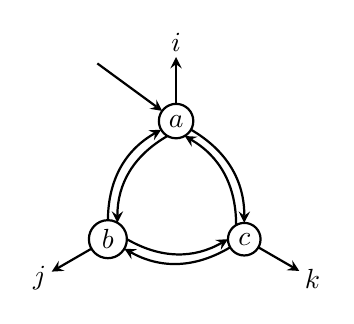
\begin{tikzpicture}[inner sep=2pt,outer sep=0pt,thick]
	\node[circle,draw] (a) at ( 90:1) {$a$} ;
	\node[circle,draw] (b) at (210:1) {$b$} ;
	\node[circle,draw] (c) at (330:1) {$c$} ;
	\node (i) at ( 90:2) {$i$} ;
	\node (j) at (210:2) {$j$} ;
	\node (k) at (330:2) {$k$} ;
	\begin{scope}[->,>=stealth]
	\draw (a.240) to[bend right] (b.60) ;
	\draw (b.0)   to[bend right] (c.180) ;
	\draw (c.120) to[bend right] (a.300) ;
	\draw (a.330) to[bend left]  (c.90) ;
	\draw (b.90)  to[bend left]  (a.210) ;
	\draw (c.210) to[bend left]  (b.330) ;
	\draw (a)--(i);
	\draw (b)--(j);
	\draw (c)--(k);
	\draw (120:2)--(a);
	\end{scope}
\end{tikzpicture}}}
\qquad
\begin{array}{l@{}l@{}l}
	    S      &{}~=~{}& \{a,b,c,i,j,k\}
\\[3pt]	s      &{}~=~{}& a
\\[3pt]	F      &{}~=~{}& \{i,j,k\}
\\[3pt]	\delta &{}~=~{}& a \mapsto \D{~b./13~,~c./13~,~i./13~}
\\[3pt]               && b \mapsto \D{~a./13~,~c./13~,~j./13~}
\\[3pt]               && c \mapsto \D{~a./13~,~b./13~,~k./13~}
\end{array}
\]
Its interpretation is as follows, writing $\term{M+N+P}$ for the term $\termcolor\lfloor\D{M./13,N./13,P./13}\rfloor$.
\[
\begin{aligned}
	\sem C &~=~ \term{({\sem{C(b)}}+{\sem{C(c)}}+i)^a}
\\	       &~=~ \term{((a+{\sem{C(b)(c)}}+j)^b + (a+{\sem{C(c)(b)}}+k)^c+i)^a}
\\         &~=~ \term{((a+(a+b+k)^c+j)^b + (a+(a+c+j)^b+k)^c+i)^a}
\end{aligned}
\]
This term is typed as follows. As in the introduction, for brevity we omit return stacks from the types.
\[
\begin{aligned}
	    \term{(a+b+k)^c}         &: \type{\e => /13a * /13b * /13k}
\\[5pt]	\term{ a+(a+b+k)^c+j}~~~ &: \type{\e => /49a * /19b * /19k + /13j}
\\[5pt] \term{(a+(a+b+k)^c+j)^b} &: \type{\e => /12a * /18k * /38j}
\\[5pt] \term{(a+(a+c+j)^b+k)^c} &: \type{\e => /12a * /18j * /38k}
\\[5pt] \term{ (a+(a+b+k)^c+j)^b + (a+(a+c+j)^b+k)^c+i}~~~ &: \type{\e => /13a * /16k * /16j * /13i}
\\[5pt] \term{((a+(a+b+k)^c+j)^b + (a+(a+c+j)^b+k)^c+i)^a} &: \type{\e => /14k * /14j * /12i}
\end{aligned}
\]
The interpretation may be illustrated as follows, where the solid edges represent the tree-shape of the probabilistic sums, while the dashed edges represent the loops.
%\[
%\begin{tikzpicture}[x=24pt,y=-24pt,inner sep=2pt,outer sep=0pt,thick]
%	\node[circle,draw] (a) at (1,0) {$a$};
%	\node[circle,draw] (b) at (0,1) {$b$};
%	\node[circle,draw] (c) at (2,1) {$c$};
%	\node[circle,draw] (d) at (0,2.4) {$c$};
%	\node[circle,draw] (e) at (2,2.4) {$b$};
%	\node (i) at (1,-1)   {$i$};
%	\node (j) at (-1,1)   {$j$};
%	\node (k) at ( 3,1)   {$k$};
%	\node (l) at (-1,2.4) {$k$};
%	\node (m) at ( 3,2.4) {$j$};
%	\begin{scope}[->,>=stealth]
%	\draw (0,-1)--(a);
%	\draw (a) to[bend right] (b);
%	\draw (a) to[bend left]  (c);
%	\draw (a) -- (i);
%	\draw (b) -- (d);
%	\draw (c) -- (e);
%	\draw (b) -- (j);
%	\draw (c) -- (k);
%	\draw (d) -- (l);
%	\draw (e) -- (m);
%	\begin{scope}[dash pattern=on 3pt off 2pt]
%	\draw (b.120) to[bend left]  (a.150);
%	\draw (c.60)  to[bend right] (a.30);
%	\draw (d.120) to[bend left]  (b.240);
%	\draw (e.60)  to[bend right] (c.300);
%	\draw (d.60)  to[bend left=10]  (a.240);
%	\draw (e.120) to[bend right=10] (a.300);
%	\end{scope}
%	\end{scope}
%\end{tikzpicture}
%\]
\[
\vc{
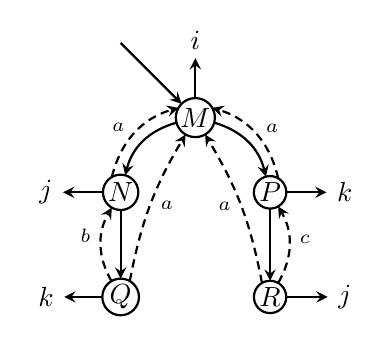
\begin{tikzpicture}[x=27pt,y=-27pt,inner sep=0.5pt,outer sep=0pt,thick]
	\node[circle,draw] (a) at (1,0) {$\term M$};
	\node[circle,draw] (b) at (0,1) {$\term N$};
	\node[circle,draw] (c) at (2,1) {$\term P$};
	\node[circle,draw] (d) at (0,2.4) {$\term Q$};
	\node[circle,draw] (e) at (2,2.4) {$\term R$};
	\node (i) at (1,-1)   {$\vphantom(i$};
	\node (j) at (-1,1)   {$~j~$};
	\node (k) at ( 3,1)   {$~k~$};
	\node (l) at (-1,2.4) {$~k~$};
	\node (m) at ( 3,2.4) {$~j~$};
	\begin{scope}[->,>=stealth]
	\draw (0,-1)--(a);
	\draw (a) to[bend right] (b);
	\draw (a) to[bend left]  (c);
	\draw (a) -- (i);
	\draw (b) -- (d);
	\draw (c) -- (e);
	\draw (b) -- (j);
	\draw (c) -- (k);
	\draw (d) -- (l);
	\draw (e) -- (m);
	\begin{scope}[dash pattern=on 3pt off 2pt]
	\draw (b.120) to[bend left]     node[pos=0.5,anchor=south east]{$\scriptstyle a~$} (a.150);
	\draw (c.60)  to[bend right]    node[pos=0.5,anchor=south west]{$~\scriptstyle a$} (a.30);
	\draw (d.120) to[bend left]     node[pos=0.5,anchor=south east]{$\scriptstyle b~$} (b.240);
	\draw (e.60)  to[bend right]    node[pos=0.5,anchor=south west]{$~\scriptstyle c$} (c.300);
	\draw (d.60)  to[bend left=10]  node[pos=0.5,anchor=west]      {$~\scriptstyle a$} (a.240);
	\draw (e.120) to[bend right=10] node[pos=0.5,anchor=east]      {$\scriptstyle a~$} (a.300);
	\end{scope}
	\end{scope}
\end{tikzpicture}
}
\qquad
\begin{array}{l@{}l}
        \term M &{}~=~\term{(N + P + i)^a}
\\[3pt] \term N &{}~=~\term{(a + Q + j)^b}
\\[3pt] \term P &{}~=~\term{(a + R + k)^c}
\\[3pt] \term Q &{}~=~\term{(a+b+k)^c}~=~\term{a+b+k}
\\[3pt] \term R &{}~=~\term{(a+c+j)^b}~=~\term{a+c+j}
\end{array}
\]
As the illustration suggests, the formalism may express any probabilistic tree with back-pointers. It may also express directed acyclic graphs, which yields a smaller interpretation of the Markov chain above, though still exponential, in the following term.
\[
	\term{ (b+c+i ; b -> a+c+j ; c -> (a+b+k ; b -> a+c+j)^c )^a }
\]
The types work out the same way.
\[
\begin{aligned}
	    \term{ b+c+i }~~~             &: \type{\e => /13b + /13c + /13i}
\\[5pt] \term{ b+c+i ; b -> a+c+j}~~~ &: \type{\e => /19a + /49c + /13i + /19j}
\\[5pt] \term{(a+b+k ; b -> a+c+j)^c} &: \type{\e => /12a + /18j + /38k}
\\[5pt] \term{ b+c+i ; b -> a+c+j ; c -> (a+b+k ; b -> a+c+j)^c}     &: \type{\e => /13a + /13i + /16j + /16k}
\\[5pt] \term{(b+c+i ; b -> a+c+j ; c -> (a+b+k ; b -> a+c+j)^c )^a} &: \type{\e => /12i + /14j + /14k}
\end{aligned}
\]


%----------------------------------------------------------------------------------------------------
\section{Moving past PAST}

The following term $\term Z$ generates a geometric series of Church numerals.
\[
	\term{Z}~=~\term{ <f>.<x>.[x].~(<n>.~([n].*~+~[[n].f].i))^i ; <m>.m }~\sim~\D{\cno./12,~\cni./14,~\cnii./18,~\dots}
\]
Let $\term M=\term{<n>.([n].*~+~[[n].f].i)}$ so that the above term is $\term{ <f>.<x>.[x].M^i ; <m>.m }$. For a given $\term N$, the term$\term{[N].M^i}$ evaluates as follows.
\[
\begin{aligned}
\term{[N].M^i}  
 ~ \rws ~ & \term{[N].M;i->M^i}
\\    = ~ & \term{[N].<n>.([n].*~+~[[n].f].i);i->M^i}
\\  \rw ~ & \term{([N].*~+~[[N].f].i);i->M^i}
\\ \sim ~ & \term{[N].* ~+~ [[N].f].M^i}
\end{aligned}
\]
The overall term $\term{ <f>.M^i ; <x>.x }$ then generates the geometric series as follows.
\[
\begin{array}{@{}r@{}l@{}}
	       & \term{ <f>.<x>.[x].M^i ; <m>.m }
\\  ~\rws~ & \term{ <f>.<x>.([x].* ; [[x].f].M^i) ; <m>.m }
\\ 	~\sim~ & \term{ <f>.<x>.[x].<m>.m ~+~ (<f>.<x>.[[x].f].M^i ; <m>;m) }
\\  ~\rw ~ & \term{ \cno ~+~ (<f>.<x>.[[x].f].M^i ; <m>;m) }
\\  ~\rws~ & \term{ \cno ~+~ (\cni ~+~ (<f>.<x>.[[[x].f].f].M^i ; <m>;m)) }
\end{array}
\]
Church numerals allow exponentiation by $\underline{m^n}=\cnn\,\cnm$. The term $\term{[\cnii].Z}$ then generates the following series.
\[
	\term{[\cnii].Z}~\sim~\D{\cni./12~,~\cnii./14~,~\cniv./18~,~..}
\]
Since Church numerals are in unary notation, the terms in the series grow exponentially. Stochastically generating a Church numeral with $\term{[\cnii].Z}$ is thus almost-surely terminating, but not \emph{positively} so.

There are two minor caveats. First, the above computations use reduction $\rw$ and equivalence $\sim$, but not evaluation on the machine. Second, since the calculus encodes constants as choices, it only admits finite datatypes. One may address both issues by introducing a natural numbers type $\type\N$ with primitive operations $\term{`+:\N\,\N=>\N}$ etc. Then the following term evaluates on the machine to return a single natural number according to the above series. (This has been confirmed experimentally.)
\[
	\term{[[0].*].[<n>.n ; [1].`+].[\cnii].Z}
\]
Note that Church numerals $\term{\cnn}$ follow a call--by--name semantics, while primitive operations on natural numbers have a call--by--value semantics. This is reflected in the base value $\term{[0].*}$ and successor function $\term{<n>.n ; [1].`+}$, which incorporate the encoding of call--by--value into call--by--name. 

It remains to show that the above terms can be typed. First, for any type $\type{s=>t}$, and indeed any type $\type{!s=>!t_I}$, the Church numerals and the term $\term Z$ can be typed as follows.
\[
\begin{aligned}
	    \term{ n }                &: \type{s=>t}
\\[5pt] \term{ f }                &: \type{(s=>t)\,s => t}
\\[5pt] \term{ [[n].f].i }        &: \type{\e => (s=>t).i}
\\[5pt] \term{ [n].*~+~[[n].f].i} &: \type{\e => (s=>t)./12* + (s=>t)./12i}
\\[5pt] \term{M}~=~\term{<n>.([n].*~+~[[n].f].i)} &: \type{(s=>t) => (s=>t)./12* + (s=>t)./12i}
\\[5pt] \term{M^i}                &: \type{(s=>t) => (s=>t)}
\\[5pt] \term{Z}~=~\term{ <f>.<x>.[x].~M^i ; <m>.m } &: \type{((s=>t)\,s => t)~(s=>t)~s~=>~t}
\end{aligned}
\]
It follows that $\term{[\cnii].Z}$ can be typed with the same type. The types of the natural number constructions are as follows.
\[
	\term{[0].* : \e=>\N} \qquad
\qquad
	\term{<n>.n ; [1]. `+ : (\e=>\N)=>\N}
\]
This gives the following overall type. 
\[
	\term{[[0].*].[<n>.n ; [1].`+].[\cnii].Z : \e=>\N}
\]
The Church numeral types $\type{((s=>t)\,s => t)~(s=>t)~s=>t}$ of $\term{\cnii}$ and $\term{Z}$ here are specialised as follows: that for $\term{\cnii}$ by replacing $\type{s=>t}$ with $\type{\e=>\N}$, and that for $\term Z$ by replacing $\type{s=>t}$ with $\type{(\e=>\N)=>\N}$.
\[
\begin{aligned}
	    \term{\cnii} &: \type{((\e=>\N)=>\N)\,(\e=>\N)=>\N}
\\[5pt]	\term{Z}     &: \type{(((\e=>\N)=>\N)\,(\e=>\N)=>\N)~((\e=>\N)=>\N)~(\e=>\N)~=>~\N}
\end{aligned}
\]
The existence of this typed term gives the following.

\begin{proposition}
The typed probabilistic FMC expresses terms that are not positively almost-sure terminating.
\end{proposition}

\section{Conclusion}


%----------------------------------------------------------------------------------------------------

\bibliography{FMC-AST}


\appendix

\subsection*{Running the machine}

\begin{example}
Below we give a successful run of the machine for our running example term, with the definition of $\term{M+N}$ unfolded to its primitives, and the trace $\bot\,\bot\,\top$.
\[
	\term{M}~=~\term{(\heads + (\tails +\,i))^i}~=~\term{(?a.a ; \top->\heads ; \bot->(?b.b ; \top->\tails ; \bot -> i))^i}
\]
\[
\begin{array}{@{(\,}r@{\,,\,}l@{\,,\,}l@{\,,\,}r@{\,)}}
             \bot\,\bot\,\top & \e &         \term{(?a.a ; \top->\heads ; \bot->(?b.b ; \top->\tails ; \bot -> i))^i} & \e
\\\hline     \bot\,\bot\,\top & \e & \phantom(\term{?a.a ; \top->\heads ; \bot->(?b.b ; \top->\tails ; \bot -> i)} & \term{(i -> M)}
\\\hline     \bot\,\bot\,\top & \e & \phantom(\term{?a.a ; \top->\heads} & \term{(\bot->(?b.b ; \top->\tails ; \bot -> i))~(i -> M)}
\\\hline     \bot\,\bot\,\top & \e & \phantom(\term{?a.a} & \term{(\top->\heads)~(\bot->(?b.b ; \top->\tails ; \bot -> i))~(i -> M)}
\\\hline           \bot\,\top & \e & \phantom(\term{\bot} & \term{(\top->\heads)~(\bot->(?b.b ; \top->\tails ; \bot -> i))~(i -> M)}
\\\hline           \bot\,\top & \e & \phantom(\term{\bot} &                \term{(\bot->(?b.b ; \top->\tails ; \bot -> i))~(i -> M)}
\\\hline           \bot\,\top & \e & \phantom(\term{?b.b ; \top->\tails ; \bot -> i} &                               \term{(i -> M)}
\\\hline           \bot\,\top & \e & \phantom(\term{?b.b ; \top->\tails} &                               \term{(\bot -> i)~(i -> M)}
\\\hline           \bot\,\top & \e & \phantom(\term{?b.b} &                               \term{(\top->\tails)~(\bot -> i)~(i -> M)}
\\\hline                 \top & \e & \phantom(\term{\bot} &                               \term{(\top->\tails)~(\bot -> i)~(i -> M)}
\\\hline                 \top & \e & \phantom(\term{\bot} &                                              \term{(\bot -> i)~(i -> M)}
\\\hline                 \top & \e & \phantom(\term{i}    &                                                          \term{(i -> M)}
\\\hline                 \top & \e & \term{(?a.a ; \top->\heads ; \bot->(?b.b ; \top->\tails ; \bot -> i))^i} & \e
\\\hline                 \top & \e & \phantom(\term{?a.a ; \top->\heads ; \bot->(?b.b ; \top->\tails ; \bot -> i)} & \term{(i -> M)}
\\\hline                 \top & \e & \phantom(\term{?a.a ; \top->\heads} & \term{(\bot->(?b.b ; \top->\tails ; \bot -> i))~(i -> M)}
\\\hline                 \top & \e & \phantom(\term{?a.a} & \term{(\top->\heads)~(\bot->(?b.b ; \top->\tails ; \bot -> i))~(i -> M)}
\\\hline                   \e & \e & \phantom(\term{\top} & \term{(\top->\heads)~(\bot->(?b.b ; \top->\tails ; \bot -> i))~(i -> M)}
\\\hline                   \e & \e & \phantom(\term{\heads} &              \term{(\bot->(?b.b ; \top->\tails ; \bot -> i))~(i -> M)}
\\\hline                   \e & \e & \phantom(\term{\heads} &                                                        \term{(i -> M)}
\\\hline                   \e & \e & \phantom(\term{\heads} & \e
\end{array}
\]
\end{example}


\subsection*{Ground terms as Markov chains}

The translation $\markov M$ from ground terms to Markov chains will take $\term M$ to a chain
\[
	\markov{M}~=~(S_M,~s_M,~F_M,~\delta_M)
\]
where internal states $S_M\less F_M$ represent subformulas and final states represent choices not captured by a later case. We consider chains modulo renaming of internal states, and when combining the translations of two terms we assume their internal states to be disjoint. To connect two chains, we use the notation $s\{t/i\}$ to rename a state, and the notation $\delta\{s/i\}$ which replaces all transitions to a (final) state $i$ with transitions to $s$.
\[
	\delta\{s/i\}(r)~=~\{~t\{s/i\}\pt p \mid t\pt p\in \delta(r)~\}
\qquad\qquad
	\begin{array}{r@{}l} i\{t/i\} &{}=t \\ s\{t/i\} &{}=s \quad (s\neq i) \end{array}
\]
The translation $\markov-$ is then as follows.
\[
\begin{aligned}
	\markov{i}      &= (\{s,i\},~s,~\{i\},~s\mapsto\D{i.1})
\\	\markov{M;i->N} &= (S_M\less\{i\}\cup S_N,~s_M,~F_M\less\{i\}\cup F_N,~\delta_M\{s_N/i\}\cup\delta_N)
\\  \markov{M^i}    &= (S_M\less\{i\},~s_M,~F_M\less\{i\},~\delta_M\{s_M/i\})
\\  \markov{?a.a}   &= (\{s,\top,\bot\},~s,~\{\top,\bot\},~s\mapsto\D{\top./12,\bot./12})
\end{aligned}
\]

\begin{example}
For the example term from the introduction, abbreviated as $\term{M^i}$ where $\term M$ is as below, the translation is as follows.
\[
	\term{M}~=~\term{?a.a ; \top->\heads ; \bot->(?b.b ; \top->\tails ; \bot -> i)}
\]
\[
\begin{array}{r@{}l}
	     \markov{?a.a}                            &{}= (\{r,\top,\bot\},~r,~\{\top,\bot\},~r\mapsto\D{\top./12,\bot./12})
\\[5pt]  \markov{?a.a ; \top->\heads}             &{}= (\{r,u,\heads,\bot\},~r,~\{\heads,\bot\},~r\mapsto\D{\bot./12,u./12}~u\mapsto\D{\heads.1})
\\[5pt]  \markov{?b.b ; \top->\tails ; \bot -> i} &{}= (\{s,v,w,\tails,i\},~s,~\{\tails,i\}, s\mapsto\D{v./12,w./12}~v\mapsto\D{\tails.1}~w\mapsto\D{i.1})
\\[5pt]  \markov{M}                               &{}= (\{r,s,u,v,w,\heads,\tails,i\},~r,~\{\heads,\tails,i\},
\\[5pt]  \multicolumn{2}{r}{ r\mapsto\D{u./12,s./12}~s\mapsto\D{v./12,w./12}~u\mapsto\D{\heads.1}~v\mapsto\D{\tails.1}~w\mapsto\D{i.1}~) }
\\[5pt]  \markov{M^i}                             &{}= (\{r,s,u,v,w,\heads,\tails\},~r,
\\[5pt]  \multicolumn{2}{r}{ r\mapsto\D{u./12,s./12}~s\mapsto\D{v./12,w./12}~u\mapsto\D{\heads.1}~v\mapsto\D{\tails.1}~w\mapsto\D{r.1}~) }
\end{array}
\]
\[
\markov{M^i}~=~\vc{
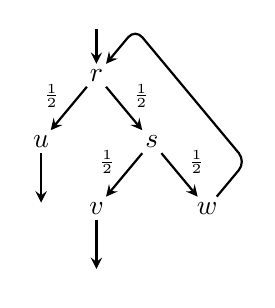
\begin{tikzpicture}[thick,x=20pt,y=24pt,outer sep=0pt,inner sep=2pt]
	\node (r) at (1,2) {$r$};
	\node (s) at (2,1) {$s$};
	\node (u) at (0,1) {$u$};
	\node (v) at (1,0) {$v$};
	\node (w) at (3,0) {$w$};
	\node (h) at (0,0) {$\termcolor\heads$};
	\node (t) at (1,-1) {$\termcolor\tails$};

	\begin{scope}[->,>=stealth]
	
	\draw (1,2.7)--(r);
	\draw (r) --node[pos=0.6,anchor=south east]{$\scriptstyle{\frac12}$} (u);
	\draw (r) --node[pos=0.6,anchor=south west]{$\scriptstyle{\frac12}$} (s);
	\draw (s) --node[pos=0.6,anchor=south east]{$\scriptstyle{\frac12}$} (v);
	\draw (s) --node[pos=0.6,anchor=south west]{$\scriptstyle{\frac12}$} (w);
	\draw (u)--(h);
	\draw (v)--(t);
	
	\draw[rounded corners] (w)--(3.7,0.7)--(1.7,2.7)--(r);
	
	\end{scope}
\end{tikzpicture}}
\]
\end{example}



\end{document}


%====================================================================================================



